\iffalse
\let\negmedspace\undefined
\let\negthickspace\undefined
\documentclass[journal,12pt,onecolumn]{IEEEtran}
\usepackage{cite}
\usepackage{amsmath,amssymb,amsfonts,amsthm}
\usepackage{algorithmic}
\usepackage{graphicx}
\usepackage{textcomp}
\usepackage{xcolor}
\usepackage{txfonts}
\usepackage{listings}
\usepackage{enumitem}
\usepackage{mathtools}
\usepackage{gensymb}
\usepackage[breaklinks=true]{hyperref}
\usepackage{tkz-euclide} % loads  TikZ and tkz-base
\usepackage{listings}



\newtheorem{theorem}{Theorem}[section]
\newtheorem{problem}{Problem}
\newtheorem{proposition}{Proposition}[section]
\newtheorem{lemma}{Lemma}[section]
\newtheorem{corollary}[theorem]{Corollary}
\newtheorem{example}{Example}[section]
\newtheorem{definition}[problem]{Definition}
%\newtheorem{thm}{Theorem}[section] 
%\newtheorem{defn}[thm]{Definition}
%\newtheorem{algorithm}{Algorithm}[section]
%\newtheorem{cor}{Corollary}
\newcommand{\BEQA}{\begin{eqnarray}}
\newcommand{\EEQA}{\end{eqnarray}}
\newcommand{\system}[1]{\stackrel{#1}{\rightarrow}}
\newcommand{\define}{\stackrel{\triangle}{=}}
\theoremstyle{remark}
\newtheorem{rem}{Remark}
%\bibliographystyle{ieeetr}
\begin{document}
%
\providecommand{\pr}[1]{\ensuremath{\Pr\left(#1\right)}}
\providecommand{\prt}[2]{\ensuremath{p_{#1}^{\left(#2\right)} }}        % own macro for this question
\providecommand{\qfunc}[1]{\ensuremath{Q\left(#1\right)}}
\providecommand{\sbrak}[1]{\ensuremath{{}\left[#1\right]}}
\providecommand{\lsbrak}[1]{\ensuremath{{}\left[#1\right.}}
\providecommand{\rsbrak}[1]{\ensuremath{{}\left.#1\right]}}
\providecommand{\brak}[1]{\ensuremath{\left(#1\right)}}
\providecommand{\lbrak}[1]{\ensuremath{\left(#1\right.}}
\providecommand{\rbrak}[1]{\ensuremath{\left.#1\right)}}
\providecommand{\cbrak}[1]{\ensuremath{\left\{#1\right\}}}
\providecommand{\lcbrak}[1]{\ensuremath{\left\{#1\right.}}
\providecommand{\rcbrak}[1]{\ensuremath{\left.#1\right\}}}
\newcommand{\sgn}{\mathop{\mathrm{sgn}}}
\providecommand{\abs}[1]{\left\vert#1\right\vert}
\providecommand{\res}[1]{\Res\displaylimits_{#1}} 
\providecommand{\norm}[1]{\left\lVert#1\right\rVert}
%\providecommand{\norm}[1]{\lVert#1\rVert}
\providecommand{\mtx}[1]{\mathbf{#1}}
\providecommand{\mean}[1]{E\left[ #1 \right]}
\providecommand{\cond}[2]{#1\middle|#2}
\providecommand{\fourier}{\overset{\mathcal{F}}{ \rightleftharpoons}}
\newenvironment{amatrix}[1]{%
  \left(\begin{array}{@{}*{#1}{c}|c@{}}
}{%
  \end{array}\right)
}
%\providecommand{\hilbert}{\overset{\mathcal{H}}{ \rightleftharpoons}}
%\providecommand{\system}{\overset{\mathcal{H}}{ \longleftrightarrow}}
	%\newcommand{\solution}[2]{\textbf{Solution:}{#1}}
\newcommand{\solution}{\noindent \textbf{Solution: }}
\newcommand{\cosec}{\,\text{cosec}\,}
\providecommand{\dec}[2]{\ensuremath{\overset{#1}{\underset{#2}{\gtrless}}}}
\newcommand{\myvec}[1]{\ensuremath{\begin{pmatrix}#1\end{pmatrix}}}
\newcommand{\mydet}[1]{\ensuremath{\begin{vmatrix}#1\end{vmatrix}}}
\newcommand{\myaugvec}[2]{\ensuremath{\begin{amatrix}{#1}#2\end{amatrix}}}
\providecommand{\rank}{\text{rank}}
\providecommand{\pr}[1]{\ensuremath{\Pr\left(#1\right)}}
\providecommand{\qfunc}[1]{\ensuremath{Q\left(#1\right)}}
	\newcommand*{\permcomb}[4][0mu]{{{}^{#3}\mkern#1#2_{#4}}}
\newcommand*{\perm}[1][-3mu]{\permcomb[#1]{P}}
\newcommand*{\comb}[1][-1mu]{\permcomb[#1]{C}}
\providecommand{\qfunc}[1]{\ensuremath{Q\left(#1\right)}}
\providecommand{\gauss}[2]{\mathcal{N}\ensuremath{\left(#1,#2\right)}}
\providecommand{\diff}[2]{\ensuremath{\frac{d{#1}}{d{#2}}}}
\providecommand{\myceil}[1]{\left \lceil #1 \right \rceil }
\newcommand\figref{Fig.~\ref}
\newcommand\tabref{Table~\ref}
\newcommand{\sinc}{\,\text{sinc}\,}
\newcommand{\rect}{\,\text{rect}\,}
%%
%	%\newcommand{\solution}[2]{\textbf{Solution:}{#1}}
%\newcommand{\solution}{\noindent \textbf{Solution: }}
%\newcommand{\cosec}{\,\text{cosec}\,}
%\numberwithin{equation}{section}
%\numberwithin{equation}{subsection}
%\numberwithin{problem}{section}
%\numberwithin{definition}{section}
%\makeatletter
%\@addtoreset{figure}{problem}
%\makeatother

%\let\StandardTheFigure\thefigure
\let\vec\mathbf


\bibliographystyle{IEEEtran}
\title{SEQUENCE AND SERIES}
\author{EE23BTECH11059- Tejas Mehtre$^{*}$% <-this % stops a space
}
\maketitle




\bigskip

\renewcommand{\thefigure}{\theenumi}
\renewcommand{\thetable}{\theenumi}
%\renewcommand{\theequation}{\theenumi}
Q: Find the sum to n terms of $3 \times 8 + 6 \times 11 + 9 \times 14 + ...$ \\
    \solution
    \fi
    \begin{table}[!ht]
    \centering
        
\begin{tabular}{|c|c|c|} 
    \hline
\textbf{Variable}& \textbf{Description}& \textbf{Value}\\\hline
       $x\brak{n}$& $n^{th}$ term of sequence& $\brak{3n+3}\brak{3n+8}u\brak{n}$\\\hline
        
  \end{tabular}
    \caption{input parameters}
\end{table}
        Sum of $n$ terms of AP is given by
        \begin{align}
            x\brak{n} &= \brak{3n+3}\brak{3n+8}u\brak{n} \\
            y\brak{n} &= x\brak{n}*u\brak{n}
        \end{align}
        \begin{equation}
   u(n) \xleftrightarrow{\mathcal{Z}} \frac{1}{(1-z^{-1})}  \quad \abs{z}>1\\ \label{eq:11.9.4.6.1.eq}
\end{equation}

\begin{equation}   
   nu(n) \xleftrightarrow{\mathcal{Z}} \frac{z^{-1}}{(1-z^{-1})^2} \quad \abs{z}>1\\ \label{eq:11.9.4.6.2.eq}
\end{equation}

\begin{equation}   
   n^2u(n) \xleftrightarrow{\mathcal{Z}} \frac{z^{-1}(1+z^{-1})}{(1-z^{-1})^3} \quad \abs{z}>1 \\ \label{eq:11.9.4.6.3.eq}
\end{equation}  

\begin{equation}
n^3u(n) \xleftrightarrow{\mathcal{Z}} \frac{z^{-1}\brak{1+4z^{-1}+z^{-2}}}{\brak{1-z^{-1}}^4} \quad \abs{z}>1 \\ \label{eq:11.9.4.6.4.eq}
\end{equation} 
\begin{align}
            \implies X\brak{z}&=9z^{-1}\frac{\brak{1+z^{-1}}}{\brak{1-z^{-1}}^3} + \frac{33\brak{z^{-1}}}{\brak{1-z^{-1}}^2} +\frac{24}{\brak{1-z^{-1}}} \abs{z}>1    \label{eq:11.9.4.6.5.eq}\\
            Y\brak{z} &= X\brak{z}U\brak{z} \label{eq:11.9.4.6.6.eq} \\
              \implies Y\brak{z}&= 9z^{-1}\frac{\brak{1+z^{-1}}}{\brak{1-z^{-1}}^4} + \frac{33\brak{z^{-1}}}{\brak{1-z^{-1}}^3} +\frac{24}{\brak{1-z^{-1}}^2} \abs{z}>1  \label{eq:11.9.4.6.7.eq}
        \end{align}
        Now from~\eqref{eq:11.9.4.6.1.eq},~\eqref{eq:11.9.4.6.2.eq},~\eqref{eq:11.9.4.6.3.eq},~\eqref{eq:11.9.4.6.4.eq},
 ~\eqref{eq:11.9.4.6.7.eq} By using  inverse Z-transform pairs,
 \begin{align}
            y\brak{n}= \brak{\frac{9n\brak{n+1}\brak{2n+1}}{6}+\frac{33n\brak{n+1}}{2}+24\brak{n+1}}u\brak{n}
        \end{align}
        $\therefore$ Sum of $n$ terms of the series whose $n^{th}$ term is given by $\brak{3n+3}\brak{3n+8}u\brak{n}$ is $(\frac{9n\brak{n+1}\brak{2n+1}}{6}+\frac{33n\brak{n+1}}{2}+24\brak{n+1})$u$\brak{n}$
        \begin{figure}[h]
    \centering
 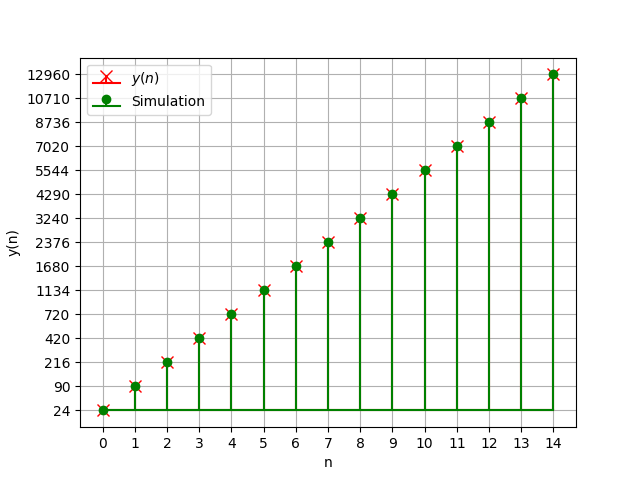
\includegraphics[width=\columnwidth]{ncert-maths/11/9/4/6/figs/plot.png}    
 \caption{Theory vs Simulation}
\end{figure}
